\documentclass{article}
\usepackage[hmargin=1in,vmargin=1in]{geometry}
\usepackage{listings}
\usepackage{color}
\usepackage{hyperref}
\usepackage{graphicx}
\usepackage{wrapfig}

% For better handling of unicode (Latin characters, anyway)
\IfFileExists{lmodern.sty}{\usepackage{lmodern}}{}
\usepackage[T1]{fontenc}
\usepackage[utf8]{inputenc}

\lstset{
    numbers=left,                   % where to put the line-numbers
    numberstyle=\small \ttfamily \color[rgb]{0.4,0.4,0.4},
                % style used for the linenumbers
    showspaces=false,               % show spaces adding special underscores
    showstringspaces=false,         % underline spaces within strings
    showtabs=false,                 % show tabs within strings adding particular underscores
    frame=lines,                    % add a frame around the code
    tabsize=4,                        % default tabsize: 4 spaces
    breaklines=true,                % automatic line breaking
    breakatwhitespace=false,        % automatic breaks should only happen at whitespace
    basicstyle=\ttfamily, %identifierstyle=\color[rgb]{0.3,0.133,0.133},   % colors in variables and function names, if desired.
    keywordstyle=\color[rgb]{0.133,0.133,0.6},
    commentstyle=\color[rgb]{0.133,0.545,0.133},
    stringstyle=\color[rgb]{0.627,0.126,0.941},
}

\hypersetup{
    colorlinks=true,
    linkcolor=blue,
    urlcolor=red,
    linktoc=all
}


\title{Rapport final de TIPE}
\author{PEREIRA Romain}
\date{4 Juin 2017}

\renewcommand*\contentsname{Sommaire}

\begin{document}

	\maketitle

	\tableofcontents

	\section*{Préambule}
		Les algorithmes de rendu graphique en temps réel consistent à générer des images numériques, qui sont calculées et affichées suffisement rapidement pour faire l'illusion de continuité sur l'œil humain.
		\newline
		\newline
		Mon travail s'est limité à l'étude de grille uniforme bi-dimensionnel sur-elevés, basée sur des champs de hauteurs. On peut ainsi simuler un relief. 
		Ce TIPE décrira leur processus de rendu, les structures de données utilisées pour les stocker en mémoire et une brève étude sur la génération de la carte de hauteur de procédure.

	\section{Introduction}


	\newpage

	\section{Corps principal}
		\subsection{Modalités d'action}
			
		\subsection{Restitution des résultats}
			\begin{figure}[!h]
				\begin{center}
					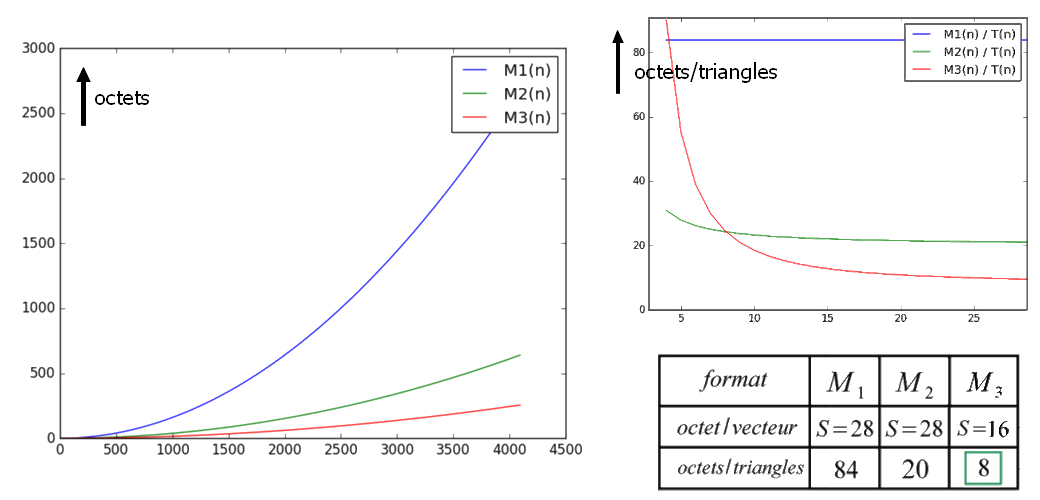
\includegraphics[width=\textwidth,height=\textheight,keepaspectratio]{../images/complexiteSpatial5.png}
				\end{center}
				\caption{Utilisation mémoire d'un terrain de coté à n points}
				\label{Utilisation mémoire du terrain}
			\end{figure}


		\subsection{Analyse - Exploitation - Discussion}


	\newpage

	\section{Conclusion générale}


	\newpage

	\section{Références}


	\newpage



\end{document}